\section{Evaluation}
\subsection{Application of Principal Component Analysis}
\label{sub:ApplicationofPrincipalComponentAnalysis}
As mentioned in Section~\ref{sub:Experiment} - \nameref{sub:Experiment}, we have four types of scenarios --
all of which we had tried to analyse to find principal components.
For each different types of scenario, we will in the following sections discuss the process of picking the principal components for analysis, what the result of the analysis is, and
how we use the generative ability of PCA to examine what each component represent variance of.

\subsubsection{Picking Principal Components}
\label{ssub:PickingPrincipalComponents}
Usually the first task after extracting principal components is to choose which of them to keep, depending on the needed variation. 
To visualize how much each principal component influenced the variation, we have plotted them using a bar chart that shows how much
of the total percentage each principal component composes (see Figure~\ref{fig:eigvplot}).
Furthermore we have plotted the cumulative sum to see how many principal components we need to have a certain percentage of variation.\\

  \begin{minipage}{\linewidth}
  \centering
  \makebox[\linewidth] {
  \begin{tabular}{cc}
      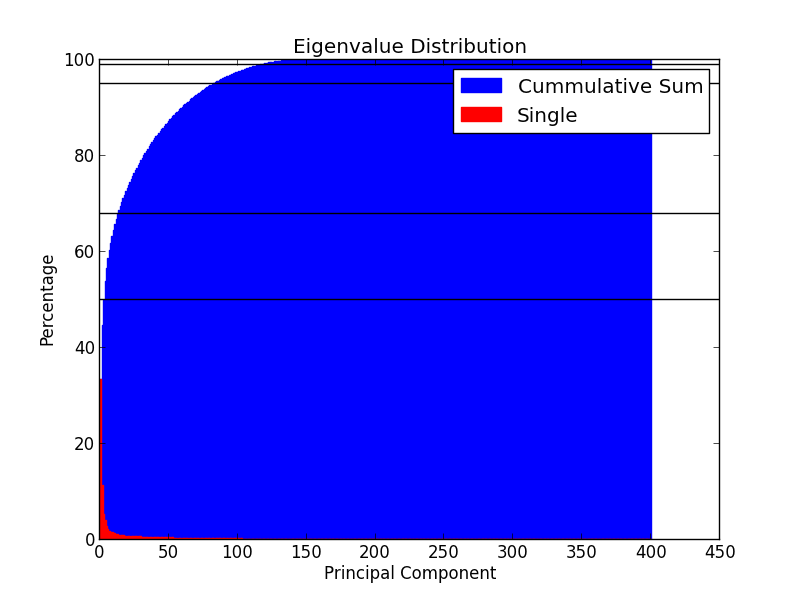
\includegraphics[width=0.5\textwidth]{NLHM-Eigenvalueplot.png}
    & 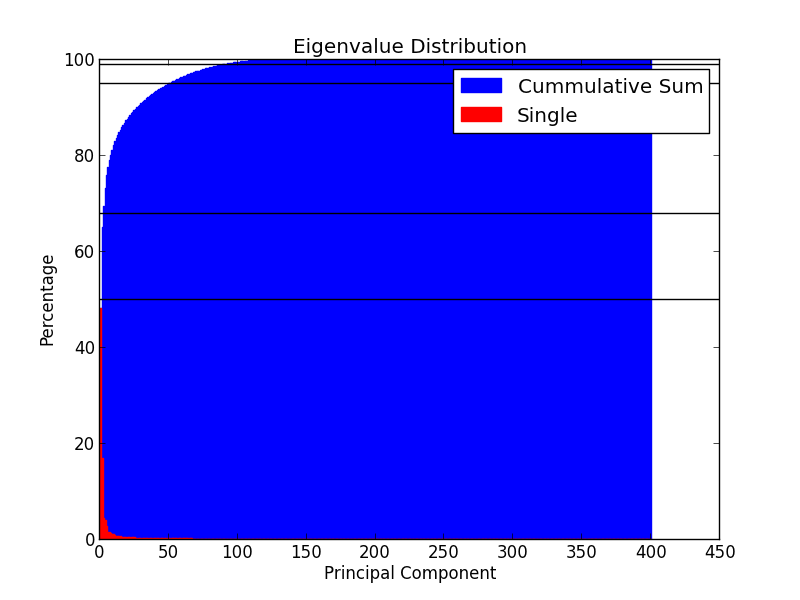
\includegraphics[width=0.5\textwidth]{NLHS-Eigenvalueplot.png} \\
      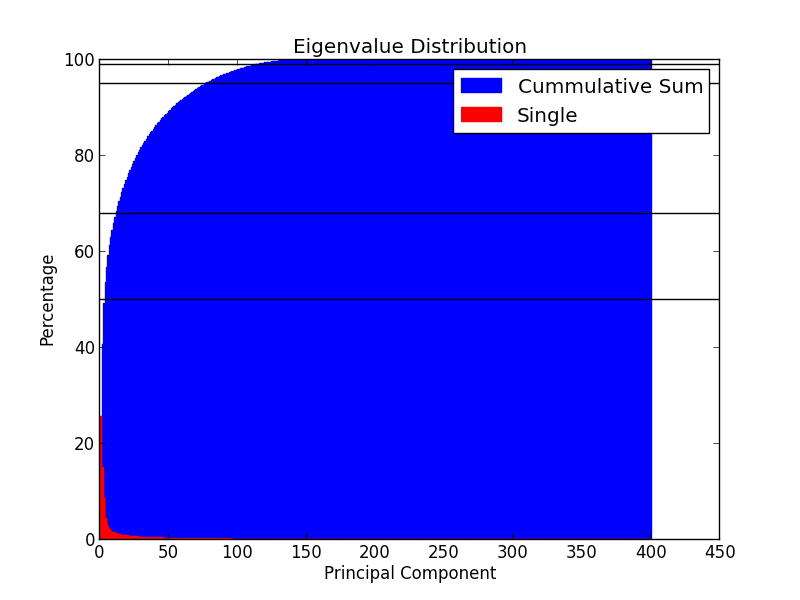
\includegraphics[width=0.5\textwidth]{WLHM-Eigenvalueplot.png}
    & 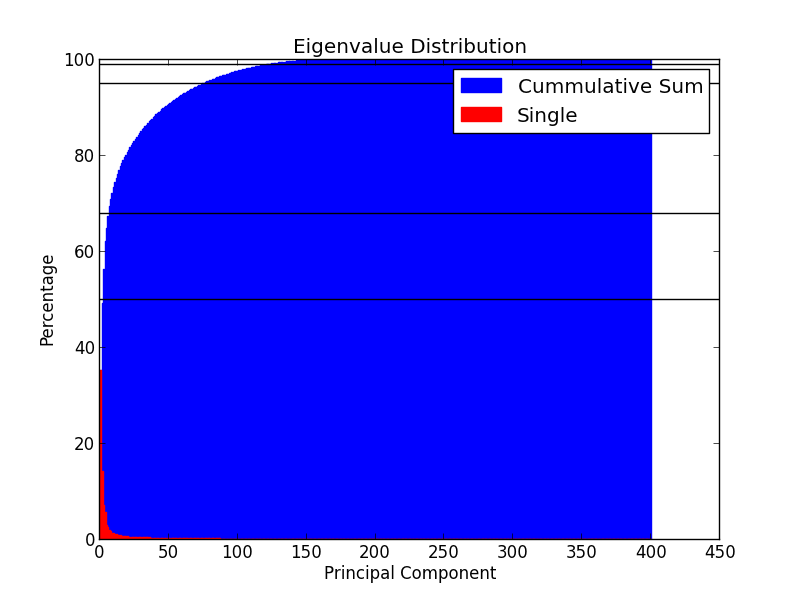
\includegraphics[width=0.5\textwidth]{WLHS-Eigenvalueplot.png}
  \end{tabular}
  }
  \captionof{figure}{Principal Components - Distribution of Variance using Eigenvalues\\
  (Left --- Right: Head Move --- Head Still, Up --- Down: No Light --- With Light)}\label{fig:eigvplot}
  \end{minipage}\\\\

As may be seen in the plots (Figure~\ref{fig:eigvplot}), in all of our test cases the first few (5-7) principal components compose almost
50\% of variation.
What is yet more interesting is that to get almost 95\% of the variation, we need almost 70 principal components in every case.
This might seem as an unusually high number, because a lot of the variations that compose the variation between 50-95\% are small in size, yet
they accumulate in size.
A possible explanation could be that our images have a lot of small variation on light, eye movement and appearance (e.g. eye colour, iris shape, etc.),
which might not useful for our purpose. This is a trade-off inherent of PCA, because it is a statistical and unsupervised method, and some of the data output
might be considered noise.

While we had examined the individual plots of all principal components to ensure that we did not exclude anything of interest, we chose to only use the most important 5 in Section~\ref{ssub:ResultData}.
This is due to the fact that while they do not represent almost all variation, they represented a comprehensible number of features while
still having a large majority. Furthermore as we will see in the next section, the features which we can use for classification, i.e. that are separable in the groups we have, are
only represented in the most important principal components.

\subsubsection{Result Data}
\label{ssub:ResultData}

\subsubsection{Generative Image Representation}
\label{ssub:GenerativeImageRepresentation}

  \begin{minipage}{\linewidth}
  \centering
  \makebox[\linewidth] {
  \begin{tabular}{ccccccc}
      \includegraphics[width=0.1\textwidth]{GeneratedImages/NLHM/PCA0-SIGMA-3.jpg}
    & \includegraphics[width=0.1\textwidth]{GeneratedImages/NLHM/PCA0-SIGMA-2.jpg}
    & \includegraphics[width=0.1\textwidth]{GeneratedImages/NLHM/PCA0-SIGMA-1.jpg}
    & \includegraphics[width=0.1\textwidth]{GeneratedImages/NLHM/PCA0-SIGMA0.jpg}
    & \includegraphics[width=0.1\textwidth]{GeneratedImages/NLHM/PCA0-SIGMA1.jpg}
    & \includegraphics[width=0.1\textwidth]{GeneratedImages/NLHM/PCA0-SIGMA2.jpg}
    & \includegraphics[width=0.1\textwidth]{GeneratedImages/NLHM/PCA0-SIGMA3.jpg} \\
      \includegraphics[width=0.1\textwidth]{GeneratedImages/NLHM/PCA1-SIGMA-3.jpg}
    & \includegraphics[width=0.1\textwidth]{GeneratedImages/NLHM/PCA1-SIGMA-2.jpg}
    & \includegraphics[width=0.1\textwidth]{GeneratedImages/NLHM/PCA1-SIGMA-1.jpg}
    & \includegraphics[width=0.1\textwidth]{GeneratedImages/NLHM/PCA1-SIGMA0.jpg}
    & 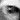
\includegraphics[width=0.1\textwidth]{GeneratedImages/NLHM/PCA1-SIGMA1.jpg}
    & 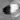
\includegraphics[width=0.1\textwidth]{GeneratedImages/NLHM/PCA1-SIGMA2.jpg}
    & 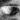
\includegraphics[width=0.1\textwidth]{GeneratedImages/NLHM/PCA1-SIGMA3.jpg} \\
      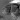
\includegraphics[width=0.1\textwidth]{GeneratedImages/NLHM/PCA2-SIGMA-3.jpg}
    & 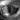
\includegraphics[width=0.1\textwidth]{GeneratedImages/NLHM/PCA2-SIGMA-2.jpg}
    & 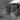
\includegraphics[width=0.1\textwidth]{GeneratedImages/NLHM/PCA2-SIGMA-1.jpg}
    & 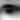
\includegraphics[width=0.1\textwidth]{GeneratedImages/NLHM/PCA2-SIGMA0.jpg}
    & 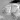
\includegraphics[width=0.1\textwidth]{GeneratedImages/NLHM/PCA2-SIGMA1.jpg}
    & 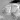
\includegraphics[width=0.1\textwidth]{GeneratedImages/NLHM/PCA2-SIGMA2.jpg}
    & 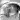
\includegraphics[width=0.1\textwidth]{GeneratedImages/NLHM/PCA2-SIGMA3.jpg} \\
      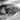
\includegraphics[width=0.1\textwidth]{GeneratedImages/NLHM/PCA3-SIGMA-3.jpg}
    & 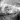
\includegraphics[width=0.1\textwidth]{GeneratedImages/NLHM/PCA3-SIGMA-2.jpg}
    & 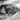
\includegraphics[width=0.1\textwidth]{GeneratedImages/NLHM/PCA3-SIGMA-1.jpg}
    & 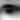
\includegraphics[width=0.1\textwidth]{GeneratedImages/NLHM/PCA3-SIGMA0.jpg}
    & 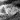
\includegraphics[width=0.1\textwidth]{GeneratedImages/NLHM/PCA3-SIGMA1.jpg}
    & 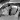
\includegraphics[width=0.1\textwidth]{GeneratedImages/NLHM/PCA3-SIGMA2.jpg}
    & 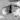
\includegraphics[width=0.1\textwidth]{GeneratedImages/NLHM/PCA3-SIGMA3.jpg} \\
      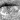
\includegraphics[width=0.1\textwidth]{GeneratedImages/NLHM/PCA4-SIGMA-3.jpg}
    & 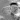
\includegraphics[width=0.1\textwidth]{GeneratedImages/NLHM/PCA4-SIGMA-2.jpg}
    & 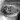
\includegraphics[width=0.1\textwidth]{GeneratedImages/NLHM/PCA4-SIGMA-1.jpg}
    & 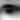
\includegraphics[width=0.1\textwidth]{GeneratedImages/NLHM/PCA4-SIGMA0.jpg}
    & 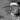
\includegraphics[width=0.1\textwidth]{GeneratedImages/NLHM/PCA4-SIGMA1.jpg}
    & 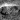
\includegraphics[width=0.1\textwidth]{GeneratedImages/NLHM/PCA4-SIGMA2.jpg}
    & 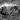
\includegraphics[width=0.1\textwidth]{GeneratedImages/NLHM/PCA4-SIGMA3.jpg}
  \end{tabular}
  }
  \captionof{figure}{No Light Head Move -- Generated PCA Images (Up --- Down: PCA 1 --- PCA 5, Left --- Right: -3$\sigma$ --- 3$\sigma$)}\label{fig:nlhmpcaimages}
  \end{minipage}\\\\


  \begin{minipage}{\linewidth}
  \centering
  \makebox[\linewidth] {
  \begin{tabular}{ccccccc}
      \includegraphics[width=0.1\textwidth]{GeneratedImages/NLHS/PCA0-SIGMA-3.jpg}
    & \includegraphics[width=0.1\textwidth]{GeneratedImages/NLHS/PCA0-SIGMA-2.jpg}
    & \includegraphics[width=0.1\textwidth]{GeneratedImages/NLHS/PCA0-SIGMA-1.jpg}
    & \includegraphics[width=0.1\textwidth]{GeneratedImages/NLHS/PCA0-SIGMA0.jpg}
    & \includegraphics[width=0.1\textwidth]{GeneratedImages/NLHS/PCA0-SIGMA1.jpg}
    & \includegraphics[width=0.1\textwidth]{GeneratedImages/NLHS/PCA0-SIGMA2.jpg}
    & \includegraphics[width=0.1\textwidth]{GeneratedImages/NLHS/PCA0-SIGMA3.jpg} \\
      \includegraphics[width=0.1\textwidth]{GeneratedImages/NLHS/PCA1-SIGMA-3.jpg}
    & \includegraphics[width=0.1\textwidth]{GeneratedImages/NLHS/PCA1-SIGMA-2.jpg}
    & \includegraphics[width=0.1\textwidth]{GeneratedImages/NLHS/PCA1-SIGMA-1.jpg}
    & \includegraphics[width=0.1\textwidth]{GeneratedImages/NLHS/PCA1-SIGMA0.jpg}
    & \includegraphics[width=0.1\textwidth]{GeneratedImages/NLHS/PCA1-SIGMA1.jpg}
    & \includegraphics[width=0.1\textwidth]{GeneratedImages/NLHS/PCA1-SIGMA2.jpg}
    & \includegraphics[width=0.1\textwidth]{GeneratedImages/NLHS/PCA1-SIGMA3.jpg} \\
      \includegraphics[width=0.1\textwidth]{GeneratedImages/NLHS/PCA2-SIGMA-3.jpg}
    & \includegraphics[width=0.1\textwidth]{GeneratedImages/NLHS/PCA2-SIGMA-2.jpg}
    & \includegraphics[width=0.1\textwidth]{GeneratedImages/NLHS/PCA2-SIGMA-1.jpg}
    & \includegraphics[width=0.1\textwidth]{GeneratedImages/NLHS/PCA2-SIGMA0.jpg}
    & \includegraphics[width=0.1\textwidth]{GeneratedImages/NLHS/PCA2-SIGMA1.jpg}
    & \includegraphics[width=0.1\textwidth]{GeneratedImages/NLHS/PCA2-SIGMA2.jpg}
    & \includegraphics[width=0.1\textwidth]{GeneratedImages/NLHS/PCA2-SIGMA3.jpg} \\
      \includegraphics[width=0.1\textwidth]{GeneratedImages/NLHS/PCA3-SIGMA-3.jpg}
    & \includegraphics[width=0.1\textwidth]{GeneratedImages/NLHS/PCA3-SIGMA-2.jpg}
    & \includegraphics[width=0.1\textwidth]{GeneratedImages/NLHS/PCA3-SIGMA-1.jpg}
    & \includegraphics[width=0.1\textwidth]{GeneratedImages/NLHS/PCA3-SIGMA0.jpg}
    & \includegraphics[width=0.1\textwidth]{GeneratedImages/NLHS/PCA3-SIGMA1.jpg}
    & \includegraphics[width=0.1\textwidth]{GeneratedImages/NLHS/PCA3-SIGMA2.jpg}
    & \includegraphics[width=0.1\textwidth]{GeneratedImages/NLHS/PCA3-SIGMA3.jpg} \\
      \includegraphics[width=0.1\textwidth]{GeneratedImages/NLHS/PCA4-SIGMA-3.jpg}
    & \includegraphics[width=0.1\textwidth]{GeneratedImages/NLHS/PCA4-SIGMA-2.jpg}
    & \includegraphics[width=0.1\textwidth]{GeneratedImages/NLHS/PCA4-SIGMA-1.jpg}
    & \includegraphics[width=0.1\textwidth]{GeneratedImages/NLHS/PCA4-SIGMA0.jpg}
    & \includegraphics[width=0.1\textwidth]{GeneratedImages/NLHS/PCA4-SIGMA1.jpg}
    & \includegraphics[width=0.1\textwidth]{GeneratedImages/NLHS/PCA4-SIGMA2.jpg}
    & \includegraphics[width=0.1\textwidth]{GeneratedImages/NLHS/PCA4-SIGMA3.jpg} \\

  \end{tabular}
  }
  \captionof{figure}{No Light Head Still -- Generated PCA Images (Up --- Down: PCA 1 --- PCA 5, Left --- Right: -3$\sigma$ --- 3$\sigma$)}\label{fig:nlhspcaimages}
  \end{minipage}\\\\

  \begin{minipage}{\linewidth}
  \centering
  \makebox[\linewidth] {
  \begin{tabular}{ccccccc}
      \includegraphics[width=0.1\textwidth]{GeneratedImages/WLHM/PCA0-SIGMA-3.jpg}
    & \includegraphics[width=0.1\textwidth]{GeneratedImages/WLHM/PCA0-SIGMA-2.jpg}
    & \includegraphics[width=0.1\textwidth]{GeneratedImages/WLHM/PCA0-SIGMA-1.jpg}
    & \includegraphics[width=0.1\textwidth]{GeneratedImages/WLHM/PCA0-SIGMA0.jpg}
    & \includegraphics[width=0.1\textwidth]{GeneratedImages/WLHM/PCA0-SIGMA1.jpg}
    & \includegraphics[width=0.1\textwidth]{GeneratedImages/WLHM/PCA0-SIGMA2.jpg}
    & \includegraphics[width=0.1\textwidth]{GeneratedImages/WLHM/PCA0-SIGMA3.jpg} \\
      \includegraphics[width=0.1\textwidth]{GeneratedImages/WLHM/PCA1-SIGMA-3.jpg}
    & \includegraphics[width=0.1\textwidth]{GeneratedImages/WLHM/PCA1-SIGMA-2.jpg}
    & \includegraphics[width=0.1\textwidth]{GeneratedImages/WLHM/PCA1-SIGMA-1.jpg}
    & \includegraphics[width=0.1\textwidth]{GeneratedImages/WLHM/PCA1-SIGMA0.jpg}
    & \includegraphics[width=0.1\textwidth]{GeneratedImages/WLHM/PCA1-SIGMA1.jpg}
    & \includegraphics[width=0.1\textwidth]{GeneratedImages/WLHM/PCA1-SIGMA2.jpg}
    & \includegraphics[width=0.1\textwidth]{GeneratedImages/WLHM/PCA1-SIGMA3.jpg} \\
      \includegraphics[width=0.1\textwidth]{GeneratedImages/WLHM/PCA2-SIGMA-3.jpg}
    & \includegraphics[width=0.1\textwidth]{GeneratedImages/WLHM/PCA2-SIGMA-2.jpg}
    & \includegraphics[width=0.1\textwidth]{GeneratedImages/WLHM/PCA2-SIGMA-1.jpg}
    & \includegraphics[width=0.1\textwidth]{GeneratedImages/WLHM/PCA2-SIGMA0.jpg}
    & \includegraphics[width=0.1\textwidth]{GeneratedImages/WLHM/PCA2-SIGMA1.jpg}
    & \includegraphics[width=0.1\textwidth]{GeneratedImages/WLHM/PCA2-SIGMA2.jpg}
    & \includegraphics[width=0.1\textwidth]{GeneratedImages/WLHM/PCA2-SIGMA3.jpg} \\
      \includegraphics[width=0.1\textwidth]{GeneratedImages/WLHM/PCA3-SIGMA-3.jpg}
    & \includegraphics[width=0.1\textwidth]{GeneratedImages/WLHM/PCA3-SIGMA-2.jpg}
    & \includegraphics[width=0.1\textwidth]{GeneratedImages/WLHM/PCA3-SIGMA-1.jpg}
    & \includegraphics[width=0.1\textwidth]{GeneratedImages/WLHM/PCA3-SIGMA0.jpg}
    & \includegraphics[width=0.1\textwidth]{GeneratedImages/WLHM/PCA3-SIGMA1.jpg}
    & \includegraphics[width=0.1\textwidth]{GeneratedImages/WLHM/PCA3-SIGMA2.jpg}
    & \includegraphics[width=0.1\textwidth]{GeneratedImages/WLHM/PCA3-SIGMA3.jpg} \\
      \includegraphics[width=0.1\textwidth]{GeneratedImages/WLHM/PCA4-SIGMA-3.jpg}
    & \includegraphics[width=0.1\textwidth]{GeneratedImages/WLHM/PCA4-SIGMA-2.jpg}
    & \includegraphics[width=0.1\textwidth]{GeneratedImages/WLHM/PCA4-SIGMA-1.jpg}
    & \includegraphics[width=0.1\textwidth]{GeneratedImages/WLHM/PCA4-SIGMA0.jpg}
    & \includegraphics[width=0.1\textwidth]{GeneratedImages/WLHM/PCA4-SIGMA1.jpg}
    & \includegraphics[width=0.1\textwidth]{GeneratedImages/WLHM/PCA4-SIGMA2.jpg}
    & \includegraphics[width=0.1\textwidth]{GeneratedImages/WLHM/PCA4-SIGMA3.jpg} \\

  \end{tabular}
  }
  \captionof{figure}{With Light Head Move -- Generated PCA Images (Up --- Down: PCA 1 --- PCA 5, Left --- Right: -3$\sigma$ --- 3$\sigma$)}\label{fig:wlhmpcaimages}
  \end{minipage}\\\\


  \begin{minipage}{\linewidth}
  \centering
  \makebox[\linewidth] {
  \begin{tabular}{ccccccc}
      \includegraphics[width=0.1\textwidth]{GeneratedImages/WLHS/PCA0-SIGMA-3.jpg}
    & \includegraphics[width=0.1\textwidth]{GeneratedImages/WLHS/PCA0-SIGMA-2.jpg}
    & \includegraphics[width=0.1\textwidth]{GeneratedImages/WLHS/PCA0-SIGMA-1.jpg}
    & \includegraphics[width=0.1\textwidth]{GeneratedImages/WLHS/PCA0-SIGMA0.jpg}
    & \includegraphics[width=0.1\textwidth]{GeneratedImages/WLHS/PCA0-SIGMA1.jpg}
    & \includegraphics[width=0.1\textwidth]{GeneratedImages/WLHS/PCA0-SIGMA2.jpg}
    & \includegraphics[width=0.1\textwidth]{GeneratedImages/WLHS/PCA0-SIGMA3.jpg} \\
      \includegraphics[width=0.1\textwidth]{GeneratedImages/WLHS/PCA1-SIGMA-3.jpg}
    & \includegraphics[width=0.1\textwidth]{GeneratedImages/WLHS/PCA1-SIGMA-2.jpg}
    & \includegraphics[width=0.1\textwidth]{GeneratedImages/WLHS/PCA1-SIGMA-1.jpg}
    & \includegraphics[width=0.1\textwidth]{GeneratedImages/WLHS/PCA1-SIGMA0.jpg}
    & \includegraphics[width=0.1\textwidth]{GeneratedImages/WLHS/PCA1-SIGMA1.jpg}
    & \includegraphics[width=0.1\textwidth]{GeneratedImages/WLHS/PCA1-SIGMA2.jpg}
    & \includegraphics[width=0.1\textwidth]{GeneratedImages/WLHS/PCA1-SIGMA3.jpg} \\
      \includegraphics[width=0.1\textwidth]{GeneratedImages/WLHS/PCA2-SIGMA-3.jpg}
    & \includegraphics[width=0.1\textwidth]{GeneratedImages/WLHS/PCA2-SIGMA-2.jpg}
    & \includegraphics[width=0.1\textwidth]{GeneratedImages/WLHS/PCA2-SIGMA-1.jpg}
    & \includegraphics[width=0.1\textwidth]{GeneratedImages/WLHS/PCA2-SIGMA0.jpg}
    & \includegraphics[width=0.1\textwidth]{GeneratedImages/WLHS/PCA2-SIGMA1.jpg}
    & \includegraphics[width=0.1\textwidth]{GeneratedImages/WLHS/PCA2-SIGMA2.jpg}
    & \includegraphics[width=0.1\textwidth]{GeneratedImages/WLHS/PCA2-SIGMA3.jpg} \\
      \includegraphics[width=0.1\textwidth]{GeneratedImages/WLHS/PCA3-SIGMA-3.jpg}
    & \includegraphics[width=0.1\textwidth]{GeneratedImages/WLHS/PCA3-SIGMA-2.jpg}
    & \includegraphics[width=0.1\textwidth]{GeneratedImages/WLHS/PCA3-SIGMA-1.jpg}
    & \includegraphics[width=0.1\textwidth]{GeneratedImages/WLHS/PCA3-SIGMA0.jpg}
    & \includegraphics[width=0.1\textwidth]{GeneratedImages/WLHS/PCA3-SIGMA1.jpg}
    & \includegraphics[width=0.1\textwidth]{GeneratedImages/WLHS/PCA3-SIGMA2.jpg}
    & \includegraphics[width=0.1\textwidth]{GeneratedImages/WLHS/PCA3-SIGMA3.jpg} \\
      \includegraphics[width=0.1\textwidth]{GeneratedImages/WLHS/PCA4-SIGMA-3.jpg}
    & \includegraphics[width=0.1\textwidth]{GeneratedImages/WLHS/PCA4-SIGMA-2.jpg}
    & \includegraphics[width=0.1\textwidth]{GeneratedImages/WLHS/PCA4-SIGMA-1.jpg}
    & \includegraphics[width=0.1\textwidth]{GeneratedImages/WLHS/PCA4-SIGMA0.jpg}
    & \includegraphics[width=0.1\textwidth]{GeneratedImages/WLHS/PCA4-SIGMA1.jpg}
    & \includegraphics[width=0.1\textwidth]{GeneratedImages/WLHS/PCA4-SIGMA2.jpg}
    & \includegraphics[width=0.1\textwidth]{GeneratedImages/WLHS/PCA4-SIGMA3.jpg} \\

  \end{tabular}
  }
  \captionof{figure}{With Light Head Still -- Generated PCA Images (Up --- Down: PCA 1 --- PCA 5, Left --- Right: -3$\sigma$ --- 3$\sigma$)}\label{fig:wlhspcaimages}
  \end{minipage}\\\\



\subsection{Creating Models for Classification}
\label{sub:CreatingModelsforClassification}
Summarize which machine learning models are used.
Compare the performance of different machine learning models.
Conclude on usability by virtue of cross-validation metrics.
\subsection{Gaze Estimation Performance on Real-World Data}
\label{sub:GazeEstimationPerformanceonReal-WorldData}
Run experiments on real-world data and talk about the actual performance metrics measured, compared to the validation metrics.
Conclude on the generalization of the calculated model in practice.

\begin{table}[h!]
\centering
\begin{tabular}{l|rrr}
\hline
\noalign{\smallskip}
 & One versus one & One versus rest & Perceptron\\
\noalign{\smallskip}
\hline
\noalign{\smallskip}
Infra-red enabled & 43.86\% & 40.35\% & 81.58\% \\
Infra-red disabled & 41.35\% & 41.35\% & 85.96\% \\
Classification results & 90\% & 78\% & 98\% \\
\hline
\end{tabular}
\caption{Test results showing percentage accuracy for the methods One versus One - Support Vector Machine (Linear Kernel), One versus Rest - Logistic Regression and Perceptron (Left/Right separability)}\label{tab:test results}
\end{table}

\begin{figure}[h!]
\centering
\includegraphics[width=0.8\textwidth]{testresultspcaplot}
\caption{PCA plot of test data on dataset WLHS.}
\label{fig:testresultspcaplot}
\end{figure}